След успешното създаване на първоначален документ, може да се пристъпи към по-сериозно оформление на текста и детайлите около него. Ще бъде разяснено логическото форматиране, как LaTeX чете входната информация, как да се модифицират шрифтовете, оформление на полета, параграфи, подравняване и цитиране.

\section{Логическо форматиране}

В самият текст на LaTeX документа не се изпълнява физическо форматиране. Авторът не се грижи дали текстът е нормален, удебелен, наклонен, подчертан или нещо друго. За целите на оформлението се използва логическо форматиране. Документът има различни фрагменти, като заглавие, име на автор, секция, подсекция и други. Физическото форматиране се извършва от LaTeX според вида на компонента и предварително заредения шаблон. 

В много редки случаи, когато става въпрос за единични изключения е допустимо да се използва и физическо форматиране, но то значително затруднява последващата поддръжка на единно оформление в документа.

Добре оформеният LaTeX документ използва физическо форматиране само в командите, които указват изпълнението на физическото форматиране.

С един много опростен документ се демонстрират най-съществените части от оформлението, като: заглавие, автор, дата и основен текст.

\begin{lstlisting}[language={[LaTeX]TeX}, caption=Инструкция за вида на документа, label=listing-0002]
\documentclass[a4paper,11pt]{article}
\end{lstlisting}

Спрямо вида на документа (Лист. \ref{listing-0002}), LaTeX зарежда необходимите инструкции и стилово оформление. В първата инструкция се задава на носителя на информация (хартия формат А4) и размера на основния текст. 

\begin{lstlisting}[language={[LaTeX]TeX}, caption={Добавяне на заглавие, автор и дата}, label=listing-0003]
\documentclass[a4paper,11pt]{article}

\title{The Story of My Life}

\author{Dessislava Gruncharova}

\date{April 21, 1979}
\end{lstlisting}

Най-съществените атрибути на един документ са заглавието, автора и дата на създаване. За всяко от трите има подходящо дефинирана инструкция (Лист. \ref{listing-0003}).

\begin{lstlisting}[language={[LaTeX]TeX}, caption=Тяло на документа, label=listing-0004]
\documentclass[a4paper,11pt]{article}

\title{The Story of My Life}

\author{Dessislava Gruncharova}

\date{April 21, 1979}

\begin{document}
\end{document}
\end{lstlisting}

След описателната част на документа следва основното изложение (Лист. \ref{listing-0004}).

\begin{lstlisting}[language={[LaTeX]TeX}, caption=Инструкция за създаване на заглавна страница, label=listing-0005]
\documentclass[a4paper,11pt]{article}

\title{The Story of My Life}

\author{Dessislava Gruncharova}

\date{April 21, 1979}

\begin{document}

\maketitle

\end{document}
\end{lstlisting}

Заглавната страница се съставя автоматично с помощта на командата maketitle (Лист. \ref{listing-0005}).

\begin{lstlisting}[language={[LaTeX]TeX}, caption=Оформяне на секция в документа, label=listing-0006]
\documentclass[a4paper,11pt]{article}

\title{The Story of My Life}

\author{Dessislava Gruncharova}

\date{April 21, 1979}

\begin{document}

\maketitle

\section{The beginning was ...}

\end{document}
\end{lstlisting}

В LaTeX възприетият принцип е документът да се разделя на секции (Лист. \ref{listing-0006}).

\begin{lstlisting}[language={[LaTeX]TeX}, caption=Текстово изложение, label=listing-0007]
\documentclass[a4paper,11pt]{article}

\title{The Story of My Life}

\author{Dessislava Gruncharova}

\date{April 21, 1979}

\begin{document}

\maketitle

\section{The beginning was ...}

The story of my life started ...

\end{document}
\end{lstlisting}

След което следва същинското текстово изложение (Лист. \ref{listing-0007}).

\begin{figure}
  \centering
  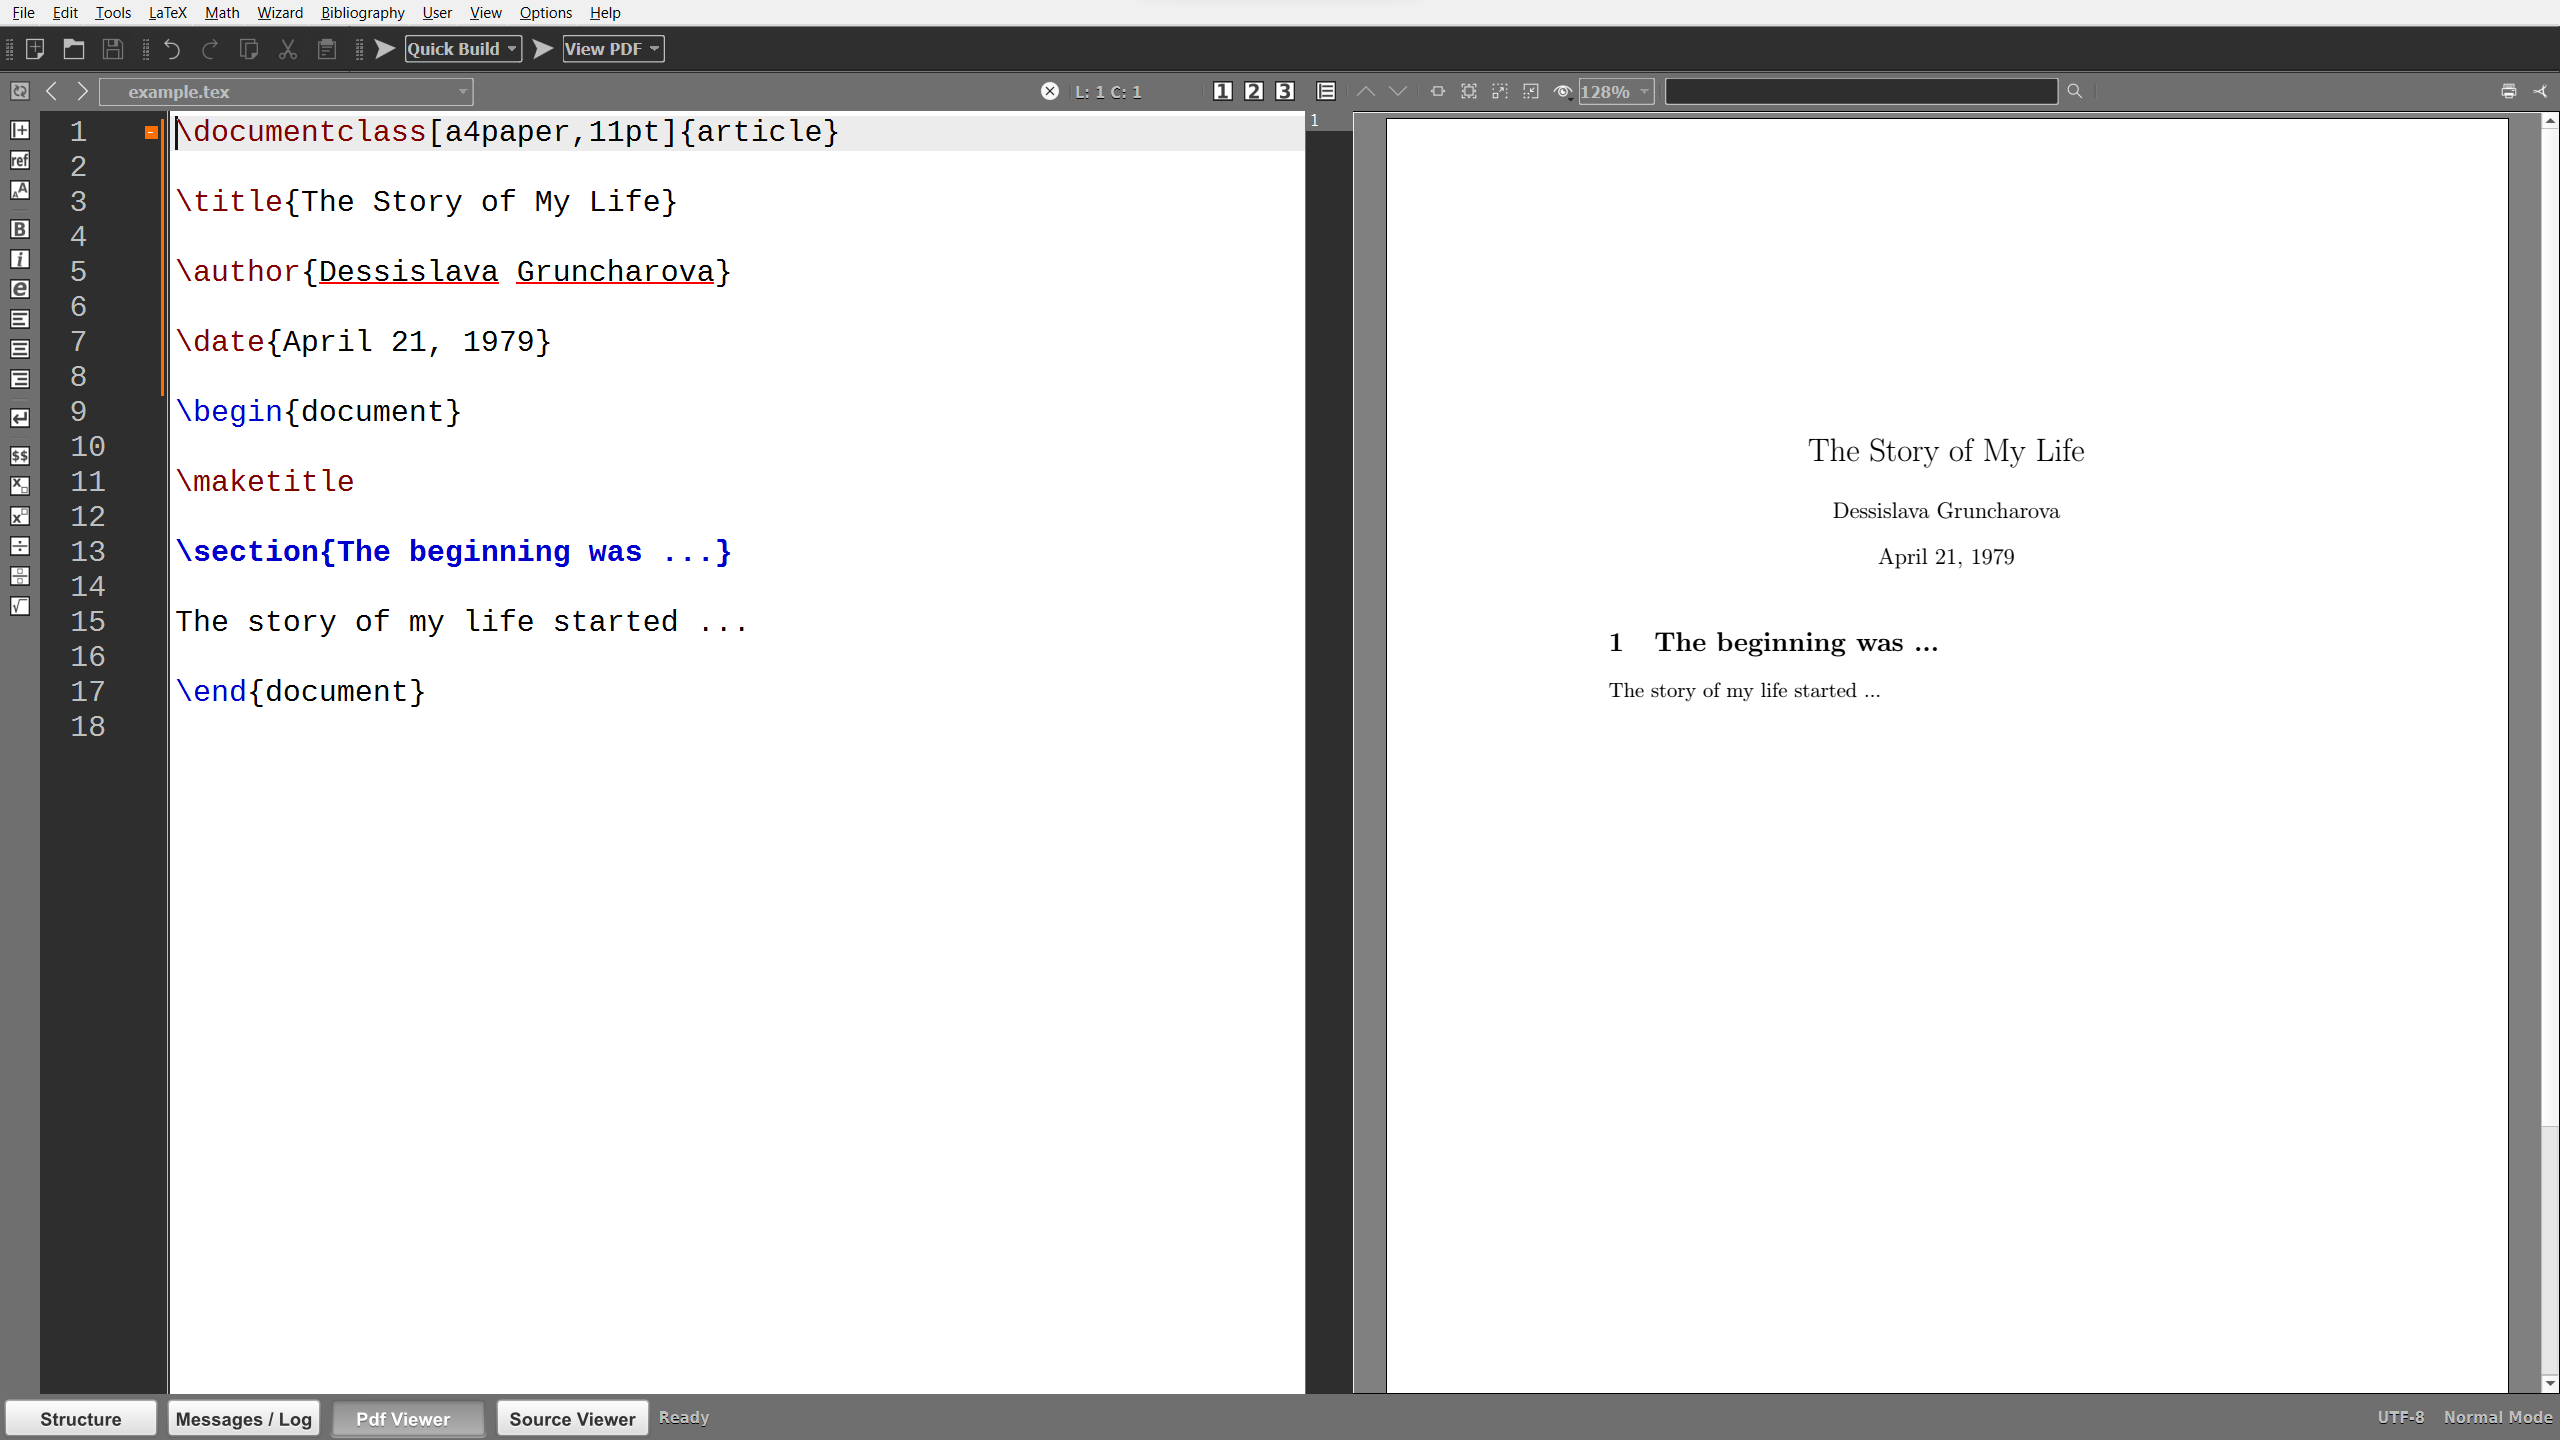
\includegraphics[width=1.0\linewidth,height=0.5\linewidth]{figure-0017.png}
  \caption{Резултат от компилацията с LaTeX}
\label{figure-0017}
\end{figure}

В резултат на извършената компилация, Texmaker предлага финалният PDF документ (Фиг. \ref{figure-0017}). Както може да се забележи, никъде не се указва размера на шрифта или графичното оформление за заглавието, автора и датата на публикуване. Всичко това е дефинирано в шаблона article. 

Важно е да се отбележи, че инструкциите в LaTeX основно започват с обратна наклонена черата, която е последвана от малки и големи букви. В повечето случай названията на инструкциите са самообясняващи се. Параметри на инструкциите се задават в къдрави скоби. Не задължителните параметри се ограждат в квадратни скоби. Освен инструкции в LaTeX има и фрагменти. Всеки фрагмент започва с ключова дума begin и завършва с ключова дума end. Както при командите, в къдрави скоби са задължителните аргументи, а в квадратни скоби са не задължителните аргументи. Във фрагмент се поставят, примерно, изображенията, листингите, таблиците и много други. 

\section{Обработка на входящата информация}



\section{Боравене с шрифтове}



\section{Оформяне на зони и параграфи}



\section{Подравняване и цитиране}



\section*{Обобщение}



